\chapter{子域和边界条件}
\label{ch:subdomains}

\index{subdomains}


\begin{quote}
到目前为止,我们只是简单地看一下如何指定边界
条件。 在本章中,我们将更仔细地研究如何指定
边界的特定部分(子域)的边界条件
如何组合多个边界条件。 我们也会看看怎么样
生成与子域的网格以及如何定义系数
在不同的子域中具有不同的值。
\end{quote}

% ========= Multiple domains and boundaries =========

\section{结合Dirichlet和Neumann条件}
\label{ch:poisson0:DN}

让我们从Chapter~\ref{ch:fundamentals}返回xPoisson问题
并看看如何扩展数学和实现来处理
Dirichlet条件与Neumann条件相结合。该
域仍然是单位广场,但现在我们设置了Dirichlet
条件$u=\ub$在左侧和右侧,$x=0$和$x=1$,而
Neumann条件

\begin{equation*}
-{\partial u\over\partial n}=g
\end{equation*}
适用于剩余的
边$y=0$和$y=1$。

\index{Neumann boundary condition}

\subsection{PDE问题}

让$\GD$和$\GN$表示边界$\partial\Omega$的部分
分别适用Dirichlet和Neumann条件。该
完整的边界值问题可以写成

\begin{alignat}{2}
    - \nabla^2 u &= f \quad&&\mbox{in } \Omega,  \\
    u &= \ub &&\mbox{on } \GD,       \\
    - {\partial u\over\partial n} &= g &&\mbox{on } \GN  \tp
\end{alignat}
再次,我们选择$u=1+x^2 + 2y^2$作为确切的解,并调整$f$,$g$和
$\ub$相应:

\begin{align*}
f(x, y) &= -6,\\
g(x, y) &= \left\lbrace\begin{array}{ll}
0, & \quad y=0,\\
4, & \quad y=1,
\end{array}\right.\\
\ub(x, y) &= 1 + x^2 + 2y^2\tp
\end{align*}

为了便于编程,我们将$g$定义为整体的一个函数
域$\Omega$,使得$g$在$y=0$和上具有正确的值
$Y=1$。 一个可能的扩展是

\begin{equation*}
g(x,y) = 4y\tp
\end{equation*}

\subsection{变化公式}

第一个任务是推导变分公式。 这一次我们不能
因为省略由零件整合产生的边界术语
$v$在$\GD$上为零。 我们有

\begin{equation*}
 -\int_\Omega (\nabla^2 u)v \dx
= \int_\Omega\nabla u\cdot\nabla v \dx - \int_{\partial\Omega}{\partial u\over
\partial n}v \ds,
\end{equation*}
因为$v=0$上$\GD$,

\begin{equation*}
- \int_{\partial\Omega}{\partial u\over
\partial n}v \ds
=
- \int_{\GN}{\partial u\over
\partial n}v \ds
= \int_{\GN}gv \ds,
\end{equation*}
通过在$\GN$上应用边界条件。
得到的弱表单读

\begin{equation}
\int_{\Omega} \nabla u \cdot \nabla v \dx
= \int_{\Omega} fv \dx - \int_{\GN} gv \ds\tp
\label{ch:poisson0:2D:DN:weak}
\end{equation}
表达这个方程
在标准符号中,$a(u,v)=L(v)$是直接的

\begin{align}
a(u, v) &= \int_{\Omega} \nabla u \cdot \nabla v \dx,
\label{ftut:poisson2:vard:a}\\
L(v) &= \int_{\Omega} fv \dx -
\int_{\GN} gv \ds\tp  \label{ftut:poisson2:vard:L}
\end{align}

\subsection{FEniCS实现}

Neumann条件如何影响实现? 让我们
重新审视我们以前的实施
\url{https://fenicsproject.org/pub/tutorial/python/vol1/ft01_poisson.py}{\nolinkurl{ft01_poisson.py}}
从部分~\ref{ch:poisson0:impl},并检查哪些更改
我们需要使xNeumann条件合并。 事实证明
只需要两个更改:

\begin{itemize}
  \item 定义Dirichlet边界的函数\texttt{boundary}必须修改。

  \item 新的边界项必须添加到\texttt{L}的表达式中。
\end{itemize}

\noindent
第一次调整可以编码为

\begin{python}
tol = 1E-14

def boundary_D(x, on_boundary):
    if on_boundary:
        if near(x[0], 0, tol) or near(x[0], 1, tol):
            return True
        else:
            return False
    else:
        return False
\end{python}
更紧凑的实现读取

\begin{python}
def boundary_D(x, on_boundary):
    return on_boundary and (near(x[0], 0, tol) or near(x[0], 1, tol))
\end{python}

\index{near@{\rm\texttt{near}}}

我们的程序的第二个调整涉及\texttt{L}的定义,
其中包括Neumann条件:

\begin{python}
g = Expression('4*x[1]', degree=1)
L = f*v*dx - g*v*ds
\end{python}
\texttt{ds}变量意味着边界积分,而\texttt{dx}
意味着域$\Omega$的整数。
不需要其他修改。

请注意,整合\texttt{*ds}是整个执行的
边界,包括Dirichlet边界。 但是,自从测试
函数\texttt{v}在Dirichlet边界上消失(因此
指定一个\texttt{DirichletBC}),积分将只包括
来自Neumann边界的贡献。

\section{设置多个Dirichlet条件}
\label{ch:poisson0:multiple:Dirichlet}

在上一节中,我们使用单个函数$\ub(x,y)$
在边界的两个部分设置Dirichlet条件。 通常是
更实用的是使用多个功能,每个子域一个
边界。 让我们再回到~\ref{ch:poisson0:DN}”部分的情况。
并根据两个Dirichlet条件重新定义问题:

\begin{alignat*}{2}
    - \nabla^2 u &= f \quad&&\mbox{in } \Omega, \\
    u &= u_{_\mathrm{L}} &&\mbox{on } \GD^{^{\mathrm{L}}}, \\
    u &= u_{_\mathrm{R}} &&\mbox{on } \GD^{^{\mathrm{R}}}, \\
    - {\partial u\over\partial n} &= g &&\mbox{on } \GN \tp
\end{alignat*}
这里,$\GD^{^{\mathrm{L}}}$是左边界$x=0$,而
$\GD^{^{\mathrm{R}}}$是右边界$x=1$。 我们注意到
$u_{_\mathrm{L}}(x, y) = 1 + 2y^2$,
$u_{_\mathrm{R}}(x, y) = 2 + 2y^2$,和
$g(x, y)=4y$。

对于$\GD^{^{\mathrm{L}}}$的边界条件,我们定义了
通常三重表达式的边界值,一个函数
定义边界的位置,以及一个\texttt{DirichletBC}对象:

\begin{python}
u_L = Expression('1 + 2*x[1]*x[1]', degree=2)

def boundary_L(x, on_boundary):
    tol = 1E-14
    return on_boundary and near(x[0], 0, tol)

bc_L = DirichletBC(V, u_L, boundary_L)
\end{python}
对于$\GD^{^{\mathrm{R}}}$的边界条件,我们写一个
类似的代码段:

\begin{python}
u_R = Expression('2 + 2*x[1]*x[1]', degree=2)

def boundary_R(x, on_boundary):
    tol = 1E-14
    return on_boundary and near(x[0], 1, tol)

bc_R = DirichletBC(V, u_R, boundary_R)
\end{python}
我们收集列表中的两个边界条件
我们可以传递给\texttt{solve}函数来计算解决方案:

\begin{python}
bcs = [bc_L, bc_R]
...
solve(a == L, u, bcs)
\end{python}

请注意,对于不依赖于$x$或$y$的边界值,我们
可以用\texttt{Constant}对象替换\texttt{Expression}对象。

\section{定义不同材质的子域}
\label{ftut:possion:2D:2mat:impl}

\index{heterogeneous media}
\index{multi-material domain}

在不同材料构成的领域解决PDE是经常发生的
遇到任务 在FEniCS中,这些问题由处理
定义域内的子域。 一个简单的例子与两个
2D中的材料(子域)将展示这一想法。 我们认为
Poisson方程的以下可变系数扩展
从章~\ref{ch:fundamentals}:

\begin{equation} \label{ch:poisson0:2D:2mat:varcoeff2}
  -\nabla \cdot \left\lbrack \kappa(x,y)\nabla u(x,y)\right\rbrack =
  f(x, y),
\end{equation}
在某些域$\Omega$。
在物理上,这个问题可以被看作是热传导的模型,
具有可变热导率$\kappa(x,y) \geq
\underline{\kappa} > 0$。

为了说明的目的,我们考虑域$\Omega =
[0,1]\times [0,1]$并将其分成两个相等的子域,如
如图~\ref{fig:subdomains}所示:

\begin{equation*}
\Omega_0 = [0, 1]\times [0,1/2],\quad
\Omega_1 = [0, 1]\times (1/2,1]\tp
\end{equation*}
我们定义$\kappa(x,y)=\kappa_0$在
$\Omega_0$和$\kappa(x,y)=\kappa_1$在$\Omega_1$,
哪里$\kappa_0, \kappa_1 > 0$被赋予常量。

%\begin{figure}[!ht]  % fig:subdomains
%  \centerline{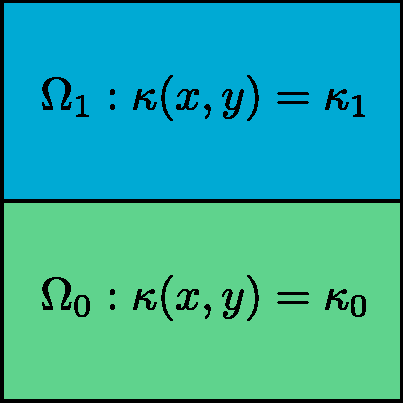
\includegraphics[width=0.5\linewidth]{fig/subdomains.pdf}}
%  \caption{
%  Two subdomains with different material parameters. \label{fig:subdomains}
%  }
%\end{figure}

变分公式可以很容易地表达在FEniCS中
如下:
\begin{python}
a = kappa*dot(grad(u), grad(v))*dx
L = f*v*dx
\end{python}
在本节的其余部分,我们将讨论不同的策略
用于将系数\texttt{kappa}定义为需要的\texttt{Expression}
两个子域中的值不同。

\subsection{使用表达式来定义子域}

实现可变系数的最简单的方法
$\kappa = \kappa(x,y)$是定义一个\texttt{Expression},它依赖于
坐标$x$和$y$。 我们以前用过\texttt{Expression}
类基于简单公式定义表达式。或者,
一个\texttt{Expression}可以被定义为一个允许更多的Python类
复杂的逻辑。 以下代码片段说明了这一点
施工:

\begin{python}
class K(Expression):
    def set_k_values(self, k_0, k_1):
        self.k_0, self.k_1 = k_0, k_1

    def eval(self, value, x):
        "Set value[0] to value at point x"
        tol = 1E-14
        if x[1] <= 0.5 + tol:
            value[0] = self.k_0
        else:
            value[0] = self.k_1

# Initialize kappa
kappa = K(degree=0)
kappa.set_k_values(1, 0.01)
\end{python}
\texttt{eval}方法在定义函数方面提供了很大的灵活性,但a
缺点是FEniCS将为Python中的每个节点\texttt{x}调用\texttt{eval}
这是一个缓慢的过程。

另一种方法是使用C++字符串表达式
以前看过,在FEniCS中效率更高。 这可以做到
使用内联如果测试:

\begin{python}
tol = 1E-14
k_0 = 1.0
k_1 = 0.01
kappa = Expression('x[1] <= 0.5 + tol ? k_0 : k_1', degree=0,
               tol=tol, k_0=k_0, k_1=k_1)
\end{python}

如果子域名定义变量系数的这种方法起作用
是可以用几何表达的简单形状
不平等。 但是,对于更复杂的子域,我们将需要
使用更一般的技术,我们将在下面看到。

\index{boundary specification (class)}

\subsection{使用网格函数来定义子域}

\index{boundary markers}
\index{MeshFunction@{\rm\texttt{MeshFunction}}}
\index{CellFunction@{\rm\texttt{CellFunction}}}
\index{FacetFunction@{\rm\texttt{FacetFunction}}}

现在我们将介绍如何指定子域$\Omega_0$和$\Omega_1$
使用更一般的技术。 这种技术涉及使用两种
在使用子域时,FEniCS中必不可少的课程:
\texttt{SubDomain}和\texttt{MeshFunction}。 考虑下面的定义
边界$x = 0$:

\begin{python}
def boundary(x, on_boundary):
    tol = 1E-14
    return on_boundary and near(x[0], 0, tol)
\end{python}
这个边界定义实际上是更通用的捷径
FEniCS概念\texttt{SubDomain}。 一个\texttt{SubDomain}是一个定义a的类
区域在空间(子域)的成员函数\texttt{inside}
它返回\texttt{True}属于子域的点
\texttt{False}对于不属于子域的点。 这是怎么回事
指定边界$x = 0$作为\texttt{SubDomain}:

\begin{python}
class Boundary(SubDomain):
    def inside(self, x, on_boundary):
        tol = 1E-14
        return on_boundary and near(x[0], 0, tol)

boundary = Boundary()
bc = DirichletBC(V, Constant(0), boundary)
\end{python}
我们注意到\texttt{Boundary}类的\texttt{inside}函数是
(几乎)与以前的边界定义相同
\texttt{boundary}功能。 技术上,我们的
类\texttt{Boundary}是一个
\emph{subclass}的FEniCS类\texttt{SubDomain}。

我们将使用两个\texttt{SubDomain}子类来定义两个子域
$\Omega_0$和$\Omega_1$:

\begin{python}
tol = 1E-14

class Omega_0(SubDomain):
    def inside(self, x, on_boundary):
        return x[1] <= 0.5 + tol

class Omega_1(SubDomain):
    def inside(self, x, on_boundary):
        return x[1] >= 0.5 - tol
\end{python}
请注意在两个测试中使用\texttt{<=}和\texttt{> =}。 FEniCS会打电话给
\texttt{inside}函数为单元格中的每个顶点确定是否
不是该单元属于特定的子域。 因此,它是
重要的是,测试对于与对齐的单元格中的所有顶点保持一致
边界。 另外,我们使用宽容来确保
内部边界上的顶点$y = 0.5$将属于两者
子域。 这是一个有点反直觉,但是是必要的
使内部边界以上和下方的细胞属于
$\Omega_0$或$\Omega_1$。

要定义变量系数$\kappa$,我们将使用一个强大的工具
FEniCS称为\texttt{MeshFunction}。 一个\texttt{MeshFunction}是一个离散的
函数可以在一组所谓的网格中进行评估
实体。 FEniCS中的网格实体是顶点,边缘,
面或细胞(三角形或四面体)。 一个\texttt{MeshFunction}在单元格上
适合代表子域(材料),而a
\texttt{MeshFunction}超过面(边或面)用于表示
外部或内部边界。 一个\texttt{MeshFunction}在单元格上
也可用于表示网格细化的边界标记。 一个
FEniCS \texttt{MeshFunction}对其数据类型(如
整数或布尔值)及其维数(0 =顶点,1 =边
等等。)。 特殊子类\texttt{VertexFunction},\texttt{EdgeFunction}等等
提供了一个特定的\texttt{MeshFunction}的容易定义
尺寸。

由于在本示例中我们需要定义$\Omega$的子域,
我们使用\texttt{CellFunction}。 构造函数
给出两个参数:(1)值的类型:\texttt{'int'}用于整数,
\verb!'size_t'! 对于非负(无符号)整数,\texttt{'double'}为真
数字和\texttt{'bool'}用于逻辑值;(2)一个\texttt{Mesh}对象。
或者,构造函数只能使用一个文件名并进行初始化
\texttt{CellFunction}从文件中的数据。

我们首先创建一个非负的\texttt{CellFunction}
整数值(\verb!'size_t'!):

\begin{python}
materials = CellFunction('size_t', mesh)
\end{python}

接下来,我们使用两个子域来\emph{mark}属于每个的单元格
子域名:
\begin{python}
subdomain_0 = Omega_0()
subdomain_1 = Omega_1()
subdomain_0.mark(materials, 0)
subdomain_1.mark(materials, 1)
\end{python}

这将将网格函数\texttt{materials}的值设置为$0$
属于所有单元格的每个单元格属于$\Omega_0$和$1$
$\Omega_1$。 或者,我们可以使用以下等效代码
标记单元格:

\begin{python}
materials.set_all(0)
subdomain_1.mark(materials, 1)
\end{python}
检查网格函数的值,看到我们确实
正确定义了我们的子域,我们可以简单地绘制网格
功能:

\begin{python}
plot(materials, interactive=True)
\end{python}
我们也可能希望以后存储网格功能的值
使用:
\begin{python}
File('materials.xml.gz') << materials
\end{python}
这可以稍后从文件中读取如下:
\begin{python}
File('materials.xml.gz') >> materials
\end{python}

现在,使用网格函数\texttt{materials}的值来定义
可变系数$\kappa$,我们创建一个FEniCS \texttt{Expression}:

\begin{python}
class K(Expression):
    def __init__(self, materials, k_0, k_1, **kwargs):
        self.materials = materials
        self.k_0 = k_0
        self.k_1 = k_1

def eval_cell(self, values, x, cell):
        if self.materials[cell.index] == 0:
            values[0] = self.k_0
        else:
            values[0] = self.k_1

kappa = K(materials, k_0, k_1, degree=0)
\end{python}

这与我们上面定义的\texttt{Expression}子类似,但是我们
使用成员函数\verb!eval_cell! 代替常规
\texttt{eval}函数。 这个版本的评估功能有一个
附加\texttt{cell}参数,我们可以用来检查我们在哪个单元格
目前正在评估功能。 我们也定义了特殊的
功能\verb!__ init__! (构造函数),以便我们可以将所有数据传递给
\texttt{Expression}创建时。

由于我们使用几何测试来定义两个\texttt{SubDomains}
对于$\Omega_0$和$\Omega_1$,\texttt{MeshFunction}方法可能看起来像
使用简单方法的不必要的复杂性
\texttt{Expression}与if-test。 但是,一般的定义是
子域可能作为\texttt{MeshFunction}(从数据文件)可用,
可能生成的网格生成过程的一部分,而不是作为一个
简单的几何测试。 在这种情况下,这里所示的方法是
推荐使用子域名的方式。

\index{CompiledSubDomain@{\rm\texttt{CompiledSubDomain}}}

\subsection{使用C ++代码片段来定义子域}

\texttt{SubDomain}和\texttt{Expression} Python类非常方便,
但是它们的使用导致每个节点从C++到Python的函数调用
在网格中。 由于这涉及到巨大的成本,我们需要做出
如果性能是一个问题,使用C ++代码。

而不是在Python中编写\texttt{SubDomain}子类,我们可以改为使用
在FEniCS中使用\texttt{CompiledSubDomain}工具来指定C++中的子域
代码,从而加快我们的代码。 考虑
类的定义\verb!Omega_0! 和\verb!Omega_1! 以上在Python。该
定义这些子域的关键字符串可以用C++语法表示
并作为参数给出\texttt{CompiledSubDomain},如下所示:

\begin{python}
tol = 1E-14
subdomain_0 = CompiledSubDomain('x[1] <= 0.5 + tol', tol=tol)
subdomain_1 = CompiledSubDomain('x[1] >= 0.5 - tol', tol=tol)
\end{python}
如所见,可以使用关键字参数指定参数。
产生的对象,\verb!subdomain_0! 和\verb!subdomain_1!,可以使用
作为普通的\texttt{SubDomain}对象。

可以应用编译的子域字符串来指定边界
好:

\begin{python}
boundary_R = CompiledSubDomain('on_boundary && near(x[0], 1, tol)',
                               tol=1E-14)
\end{python}

也可以提供C++字符串(不带参数)
直接作为\texttt{DirichletBC}的第三个参数
构造一个\texttt{CompiledSubDomain}对象:

\begin{python}
bc1 = DirichletBC(V, value, 'on_boundary && near(x[0], 1, tol)')
\end{python}

Python \texttt{Expression}类也可以使用C ++重新定义更多
高效的代码。 再次考虑上面的class \texttt{K}的定义
对于变量系数$\kappa = \kappa(x)$。 这可以使用a重新定义
C++代码片段和关键字\texttt{cppcode}到常规FEniCS
\texttt{Expression}类:

\begin{python}
cppcode = """
class K : public Expression
{
public:

  void eval(Array<double>& values,
            const Array<double>& x,
            const ufc::cell& cell) const
  {
    if ((*materials)[cell.index] == 0)
      values[0] = k_0;
    else
      values[0] = k_1;
  }

  std::shared_ptr<MeshFunction<std::size_t>> materials;
  double k_0;
  double k_1;

};
"""

kappa = Expression(cppcode=cppcode, degree=0)
kappa.materials = materials
kappa.k_0 = k_0
kappa.k_1 = k_1
\end{python}
